\paragraph{Simultator Sickness Questionnaire}

Since the SSQ is a standardized method for simulator sickness evaluation, 
results will be presented first.
Results for the questionnaire before conducting the study were a mean of 7.63 for
nausea (sd = 10.45), 14.96 for occulomotor (sd = 19.07),
11.14 for disorientation (sd = 18.15)  resulting in 
a total SSQ score of 13.46 (sd = 18.05).
After playing through the scenarios, values channged to
a mean of 13.36 for
nausea (sd = 20.9), 17.95 for occulomotor (sd = 24.58),
27.84 for disorientation (sd = 40.58) resulting in 
a total SSQ score of 21.69 (sd = 29.97).

\begin{figure}[ht]
    \centering
    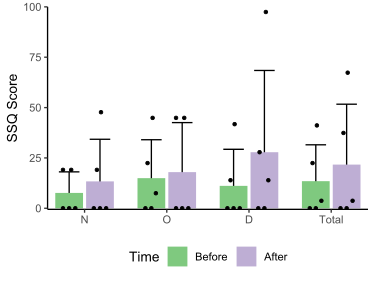
\includegraphics[width=0.7\linewidth]{images/evaluation/VR-SSQ.png}
    \caption{\label{fig::ssq}Results of the paired t-test,
    taken before and after playing through the scenarios of the study.}
\end{figure}

Results of the paired t-test, as depicted in Figure \ref{fig::ssq},
show that 
there is no significant difference between the total SSQ 
score before and after the evaluation (p = 0.602).
However, one of the participants reported a significant deterioration
of wellbeing, especially related to nausea.

\paragraph{System Usability Scale}

\begin{table}[ht]
    \centering
    \begin{tabular}{llllllllllll}
    \rowcolor[HTML]{FFFFFF} 
                         & \multicolumn{10}{c}{\cellcolor[HTML]{FFFFFF}\textbf{Question}}                                                                             & \textbf{}          \\
    \rowcolor[HTML]{FFFFFF} 
    \textbf{Participant} & \textbf{q1} & \textbf{q2} & \textbf{q3} & \textbf{q4} & \textbf{q5} & \textbf{q6} & \textbf{q7} & \textbf{q8} & \textbf{q9} & \textbf{q10} & \textbf{SUS Score} \\
    \rowcolor[HTML]{FFFFFF} 
    \textbf{1}           & 5           & 1           & 5           & 1           & 4           & 2           & 5           & 1           & 5           & 3            & \textbf{90,0}      \\
    \rowcolor[HTML]{FFFFFF} 
    \textbf{2}           & 5           & 2           & 4           & 1           & 5           & 1           & 4           & 1           & 4           & 2            & \textbf{87,5}      \\
    \rowcolor[HTML]{FFFFFF} 
    \textbf{3}           & 2           & 4           & 5           & 3           & 4           & 3           & 5           & 4           & 4           & 2            & \textbf{60,0}      \\
    \rowcolor[HTML]{FFFFFF} 
    \textbf{4}           & 5           & 2           & 5           & 4           & 3           & 2           & 4           & 2           & 4           & 4            & \textbf{67,5}      \\
    \rowcolor[HTML]{FFFFFF} 
    \textbf{5}           & 3           & 1           & 5           & 1           & 5           & 1           & 4           & 1           & 5           & 1            & \textbf{92,5}      \\
    \rowcolor[HTML]{FFFFFF} 
                         & \multicolumn{10}{l}{\cellcolor[HTML]{FFFFFF}}                                                                                              & \textbf{}          \\
    \rowcolor[HTML]{FFFFFF} 
                         & \multicolumn{10}{r}{\cellcolor[HTML]{FFFFFF}Total SUS Score}                                                                               & \textbf{79,5}      \\
    \rowcolor[HTML]{FFFFFF} 
                         & \multicolumn{10}{r}{\cellcolor[HTML]{FFFFFF}Std. Dev}                                                                                      & \textbf{14,7}      \\
    % \rowcolor[HTML]{FFFFFF} 
    %                      & \multicolumn{10}{r}{\cellcolor[HTML]{FFFFFF}95\% Confidence Interval}                                                                      & 12,90826           \\
    % \rowcolor[HTML]{FFFFFF} 
    %                      & \multicolumn{10}{r}{\cellcolor[HTML]{FFFFFF}Upper CI Bound}                                                                                & 86,0               \\
    % \rowcolor[HTML]{DCE6F1} 
    %                      & \multicolumn{10}{r}{\cellcolor[HTML]{DCE6F1}Lower CI Bound}                                                                                & 73,0              
    \end{tabular}
    \caption{Results of the SUS}
    \label{tab::sus}
\end{table}

The results for system usability are depicted in Table \ref{tab::sus}.
The system was generally perceived as being usable with a total
score of 79,5 points. The subjective usability is above the
average of 68 points \cite{sauro2016quantifying}.
However, the standard deviation is also above the average of 
12,5 points \cite{sauro2016quantifying}, with 14,7 points.
3 out of 5 participants rated the SUS very high,
with 87,5 to 92,5 points. 
From the high standard deviation it follows that the rest of the 
participants perceived the usability as poor. 
All participants felt, that the system was easy to use,
as they rated questions q3, q7 and q9 especially high.
The participants no longer share the same opinions on the other questions, 
and the three well-scoring participants clearly separate 
in sentiment from the others.
With only one of the participants agreeing that the system
was cumbersome to use (q8), and another one feeling that they
would need a technical person to understand the system (q4),
the majority of participants felt confident in using the system on their own.

\paragraph{Application-specific questionnaire}
The results of the application-specific questionnaire are depicted
in Figures \ref{fig::vrSet1} and \ref{fig::vrSet2}.
Here, questions Q1-Q15 focus on features concerning
pre-operative planning and training, 
which were implemented in the context of this thesis.
Questions Q16-Q20 focus on general VR-related
questions in context of this application.

\begin{sidewaysfigure}[ht]
    \centering
    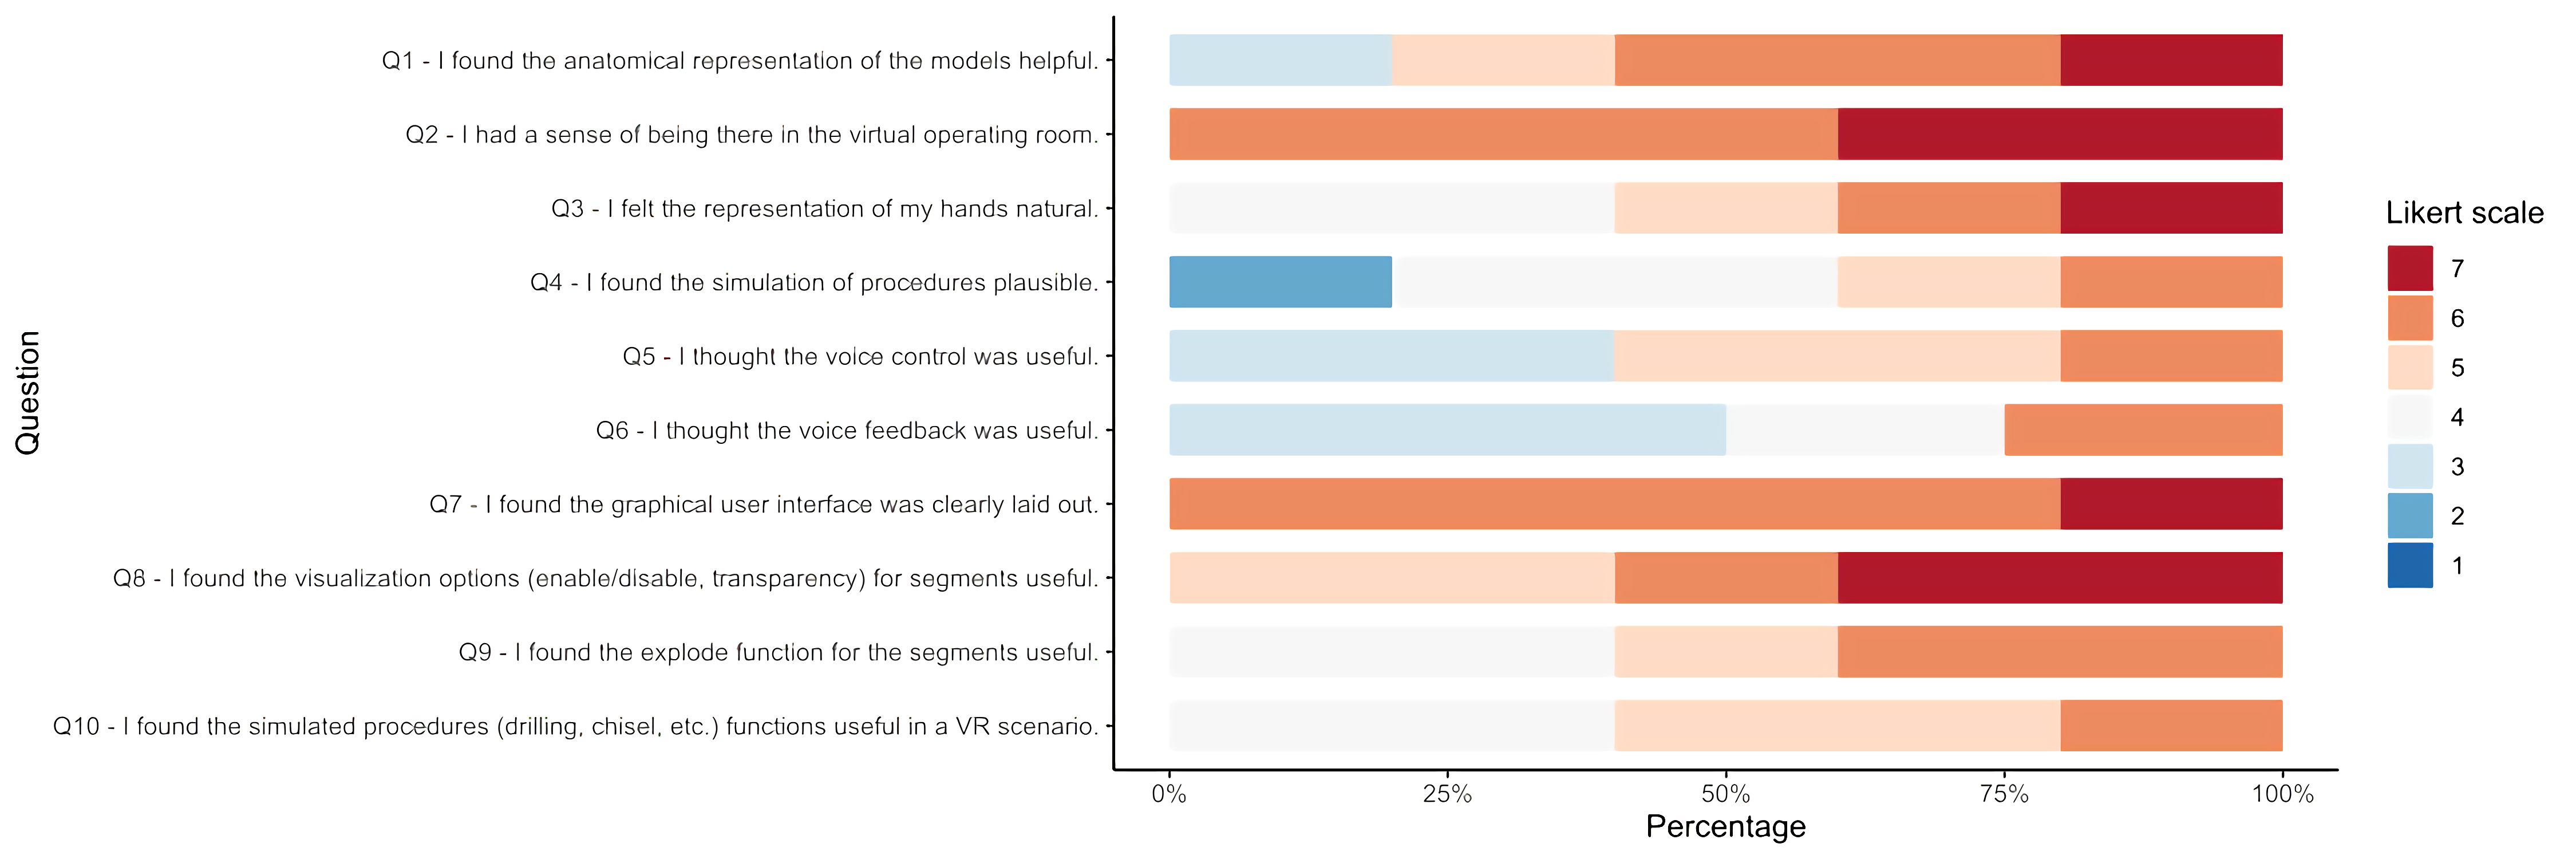
\includegraphics[width=\linewidth]{images/evaluation/VR-SET1.png}
    \caption{\label{fig::vrSet1}Results of the application-specific questionnaire (part 1).}
\end{sidewaysfigure}

\begin{sidewaysfigure}[ht]
    \centering
    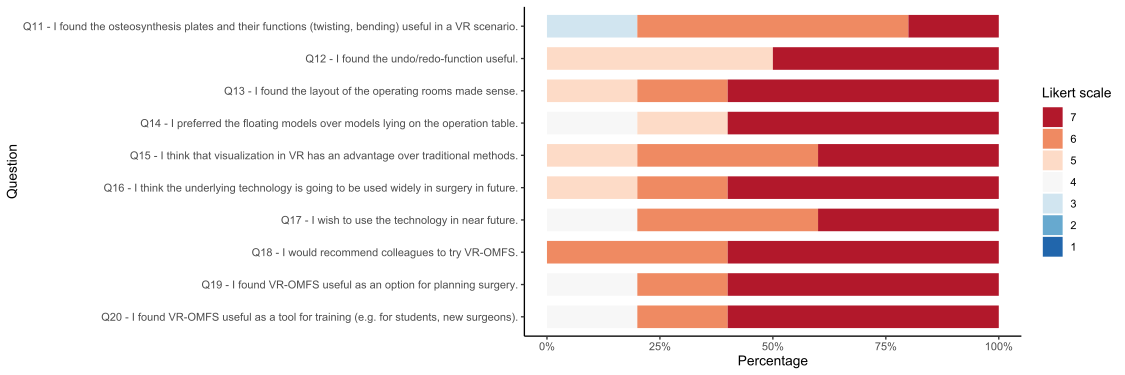
\includegraphics[width=\linewidth]{images/evaluation/VR-SET2.png}
    \caption{\label{fig::vrSet2}Results of the application-specific questionnaire (part 2).}
\end{sidewaysfigure}

The general consensus towards the abstract simulation of procedures,
as depicted in Section \ref{sec::Features}, was perceived as 
being mediocre. None of the participants rated the plausability
of simulated procedures with the highest rating.
However, the worst rating was also not given. The anatomical 
representation of patients' anatomy was generally rated as being
helpful, while one of the participants slightly disagreed. 
However, visualization options and usefulness of simulated procedures
had generally positive feedback. Especially toggling and setting the 
transparency of individual segments was being perceived as particularly
useful.
The presence of being in the virtual operating room was rated
especially high. Additionally, user's feedback on the representation
of their virtual hands was positive. 
The GUI was perceived as being well structured.
Voice related features, meaning feedback and control, have been
perceived as being mediocre. 
Undo and redo functions were unanimously found helpful.
The simulation of the osteosynthesis plates with focus on
twisting and bending functionalities were also rated high,
although one participant felt they were not useful.
The layout of the operating room as well as the floating patient
models were perceived positively. 
\\ The general VR-related feedback in context of this application
was overwhelmingly positive. 
Participants would unanimously recommend colleagues to try
out the application. Additionally, they would like to see
more of the underlying technology in the future.
The various tools of the application were found to be 
useful options for pre-operative planning and training.

\paragraph{General feedback}
As already mentioned, the last page of the questionnaire served as 
an opportunity to give general feedback and thoughts.
\\ The majority of participants stressed that they would have liked
a more realistic simulation of procedures. It was criticized,
that the procedures did not have any real effect on the anatomy
of the patient model. One participant also mentioned,
that a realistic simulation of the cutting of skin would have
been beneficial. 
\\ One participants noted, that he would like
a visual walking option instead of teleporting. Another participant
criticized that touching the GUI with their virtual hands 
was confusing, since there was no real haptic feedback when 
touching GUI components. 
\\ The interaction options 
and learnability of the system were praised by the majority of 
participants. The immersion of the application was also praised,
particularly that the application was responsive and had no 
delay.